\begin{figure}[htbp]
  \centering
  
  % Define common styles and coordinate macros
  \newcommand{\drawTetragon}{
    \coordinate (A) at (0, 0.5);
    \coordinate (B) at (1.2, 2.5);
    \coordinate (C) at (3.2, 2.0);
    \coordinate (D) at (2.8, 0.2);

    % Draw the quadrilateral
    \draw[thick] (A) -- (B) -- (C) -- (D) -- cycle;

    % Place vertex dots and labels
    \fill (A) circle (1.5pt) node[left] {$A$};
    \fill (B) circle (1.5pt) node[above left] {$B$};
    \fill (C) circle (1.5pt) node[above right] {$C$};
    \fill (D) circle (1.5pt) node[below right] {$D$};
  }

  % 1. Arbitrary Tetragon ABCD
  \begin{subfigure}[b]{0.31\textwidth}
    \centering
    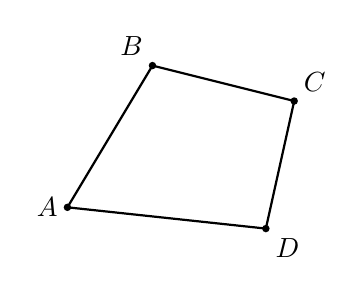
\begin{tikzpicture}[scale=0.9]
      \drawTetragon
    \end{tikzpicture}
    \caption{Arbitrary Tetragon $ABCD$}
  \end{subfigure}
  \hfill
  % 2. Tetragon with Diagonal AC
  \begin{subfigure}[b]{0.31\textwidth}
    \centering
    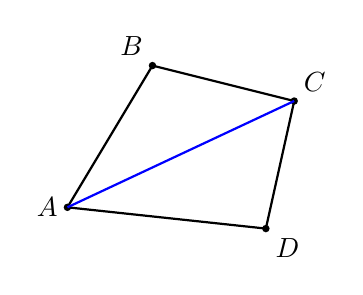
\begin{tikzpicture}[scale=0.9]
      \drawTetragon
      \draw[thick, blue] (A) -- (C);
    \end{tikzpicture}
    \caption{Tetragon with Diagonal $AC$}
  \end{subfigure}
  \hfill
  % 3. Tetragon with Diagonal BD
  \begin{subfigure}[b]{0.31\textwidth}
    \centering
    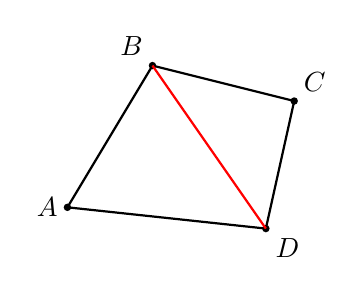
\begin{tikzpicture}[scale=0.9]
      \drawTetragon
      \draw[thick, red] (B) -- (D);
    \end{tikzpicture}
    \caption{Tetragon with Diagonal $BD$}
  \end{subfigure}

  \caption{Comparison of Tetragon $ABCD$ with its diagonals}
\end{figure}

